\chapter{The Software Project Architecture}\label{chap:arch}

In this chapter, we outline the conceptual design of the software package.
We describe individual parts and how they interact.
We talk about commands to execute the project.
\todoA{finish this when the chapter is really ready}


The software package was designed and developed with extensibility in mind.
It allows easily adding new features, specifying different subsets of data and converting them into various format without breaking older experiments.
Various libraries are utilized for both higher performance and easier maintainability.
Abstract classes are utilized for defining clear API and allow easy addition of new algorithms.

A special configuration file is utilized allowing to change the behaviour without touching the code base.
All classes and files have documentation strings which should be sufficient for detailed understanding.
In this chapter, we only describe the high-level overview.

A conceptual overview is outlined in \autoref{fig:conceptual_design}.
The flow of the programme is top to bottom.
Ellipses represent processes, rectangles data and cut rectangles input data.
The output is represented by \textit{result}.

First, unused reviews are dropped resulting in \textit{filtered reviews}.
Filtered reviews are added the information about the businesses they belong to in \texttt{join}.
The result is stored in the \textit{instance file}.

In addition to the provided data, external text analysis is used.
Entities and sentiment are extracted from all reviews and
subsequently not used reviews are dropped resulting in \textit{filtered entities and sentiment}.

The two files \textit{instance file} and \textit{filtered entities and sentiment} 
are used for generating instances with all necessary data represented by \textit{full instances}.
Full instances are split into pairs of training and testing sets for k-fold cross validation.

Next, \textit{experiments file} is loaded.
Information about classifier configuration is used to generate samples from \textit{train and test sets pairs}.
The samples have exactly the needed features for the particular classifier and necessary preprocessing is done
resulting in \textit{preprocessed instances}.

Preprocessed instances are used for training and testing the classifier.
Testing set is used for evaluating.
Evaluation results are saved into output files as defined in \textit{graphs specification} extracted from
the \textit{experiments file}.


\begin{figure}[h!]
    \centering
	\includegraphics[width=\textwidth]{figures/conceptual_design.png}
	\caption{Conceptual Design}\label{fig:conceptual_design}
\end{figure}






\section{Parts Overview}

The project is implemented in three separate parts as shown in \autoref{fig:arch_process}.
\texttt{Prepare data} creates the instances file and corresponds to rectangle A in \autoref{fig:conceptual_design}.
\texttt{Add Geneea analysis} corresponds to rectangle B --- it creates filtered entities and sentiment.
The last part \texttt{Run experiments} does the entire training, evaluating and creating statistics process.
It is represented by rectangle C.
Subset of the last part is devoted to running the experiments; \texttt{run experiments} corresponds to rectangle D.

We describe each part in a separate subsection.

\begin{figure}[h]
    \centering
	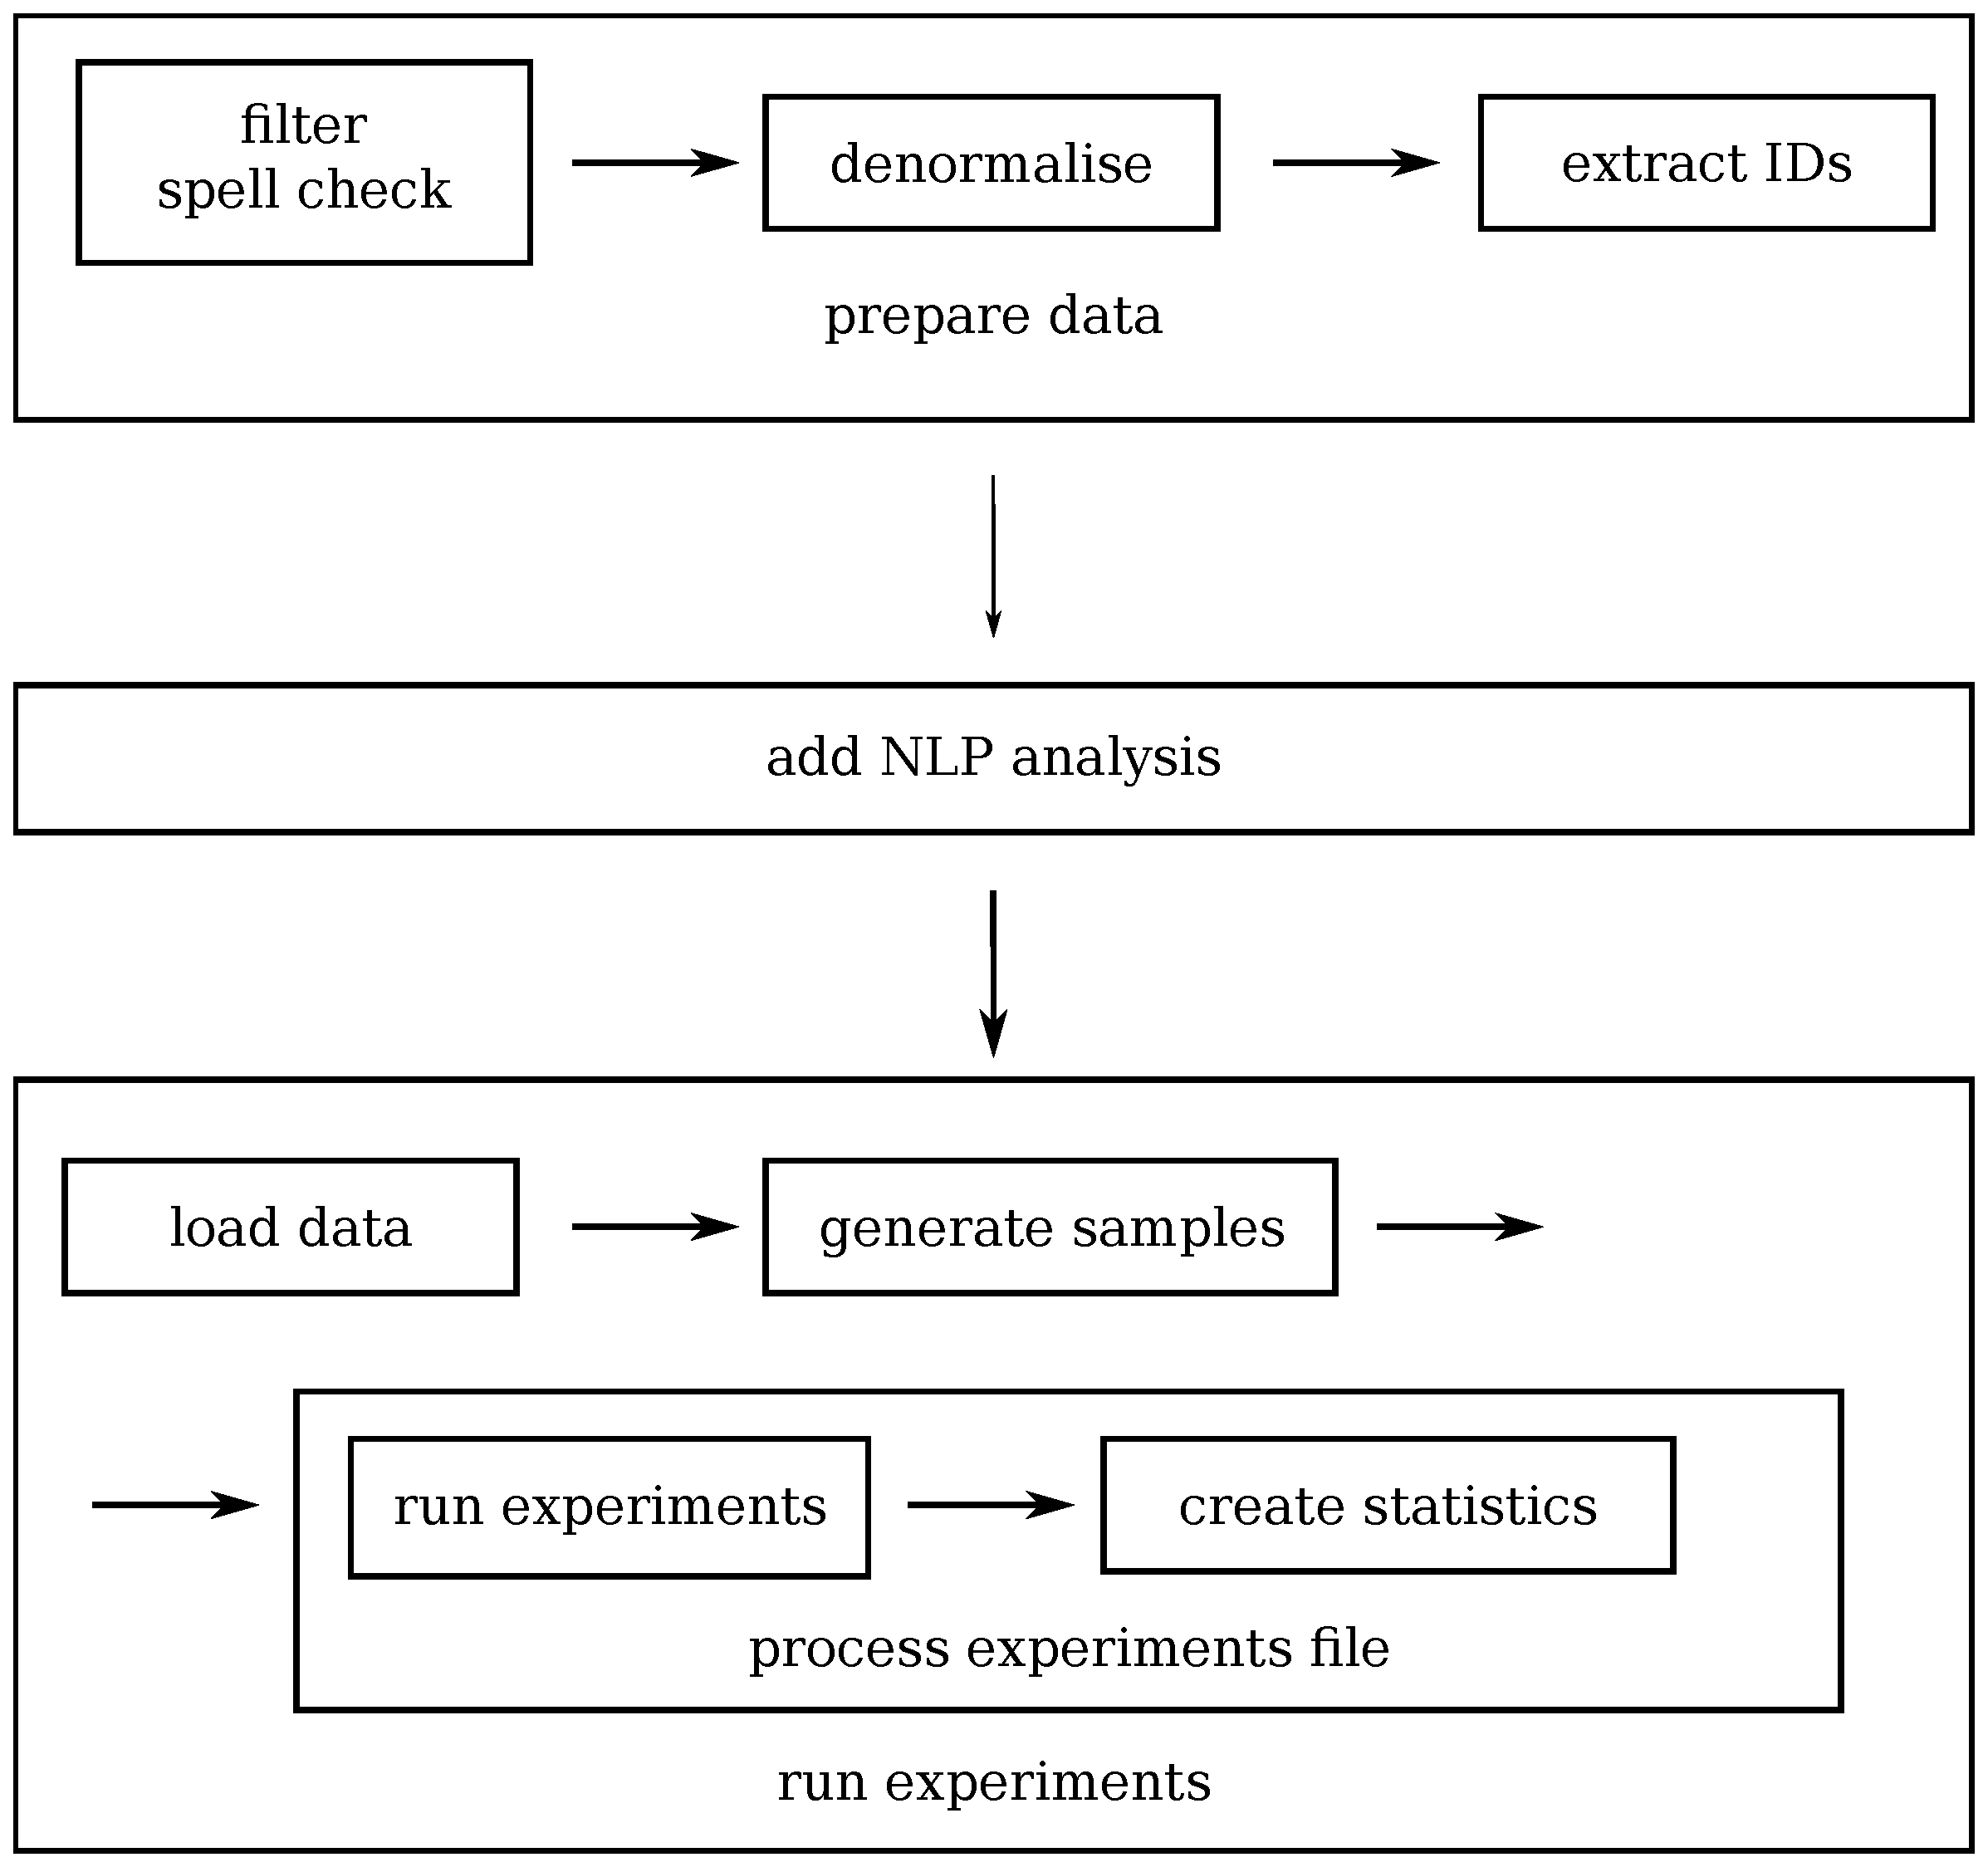
\includegraphics[width=10cm]{figures/arch_process.eps}
	\caption{Architecture Design}\label{fig:arch_process}
\end{figure}


\subsection{Data Preparation} 

All scripts for preparing data are in the folder \texttt{denormalization}.
These scripts take the dataset and produce an instance file.
Filtering of reviews as specified in \autoref{app:prepr} is done.
Because reviews are processed through the spellchecker for filtering,
the output is added into data as a byproduct.
In \texttt{denormalize}, businesses are joined.

At the end, in addition to the instance file, ID file is also created.
It contains extracted IDs from the instance file.
This is used to tell the Geneea analyzer what reviews are needed to save bandwidth,
because the Geneea analysis is performed on a remote server.

\subsection{Geneea Analysis}

Geneea analysis uses external tools for extracting more linguistics features.
Thorough description can be found in \autoref{app:geneea}.
The analysis extracts entities and sentiment from all reviews.
Subsequently, it takes filtered reviews in the form of ID file to drop all unnecessary data.
The result is stored in a file, which has to be transferred to the local computer in order to be able to continue with the next part.


\subsection{Run Experiments}

This entire part is handled by \texttt{process\_data.py}.


\subsubsection{Load Data}

Class \texttt{Data} is created by \texttt{process\_data.py}.
It is defined in file \texttt{load\_data.py} and is used for loading data.
It stores raw data in Pandas DataFrame to achieve easier manipulation without compromising performance.

\texttt{process\_data.py} uses this class for generating samples and getting the right data.
Whenever a new sample is generated, the raw data is filtered out and split into chunks.
The chunks are stored in an instance of \texttt{Sample}.
\texttt{Sample} still keeps only raw data.
Anytime a dataset is accessed all features are regenerated to ensure everything is up-to-date.


\subsubsection{Conduct Experiments}

Once all data is loaded in the memory, experiments are conducted.
The file \texttt{process\_data.py} reads the experiments file, create instances of classifiers and preprocessors.
These instances are then fed with data from the instance of \texttt{Sample}.
All tasks are guaranteed to be run on the exactly same data to ensure comparability of results.

Both training and testing is implemented by a pipeline.
The units of the pipeline are preprocessors and a classifier.
The preprocessors are in the same order as in the experiment file.
A preprocessor must be defined in the directory \texttt{preprocessors} and be a child of \texttt{preprocessors/preprocessingbase.py}.
Also, its name must be added into \texttt{preprocessors/\_\_init\_\_.py}.

Since the input and output formats of the pipeline units are arbitrary,
it is up to the user to ensure compatibility of adjacent units.
This holds except for the input of the first preprocessor and the output of the classifier.
The first preprocessor in the pipeline must take feature\_dict with possibly additional data specified in \texttt{extra\_data} as returned by \texttt{load\_data.Data.get\_feature\_dict}.
The classifier must return the predicted label.
The output of training is not stored.
Note that for most classifiers, it is needed to run conversion to matrix as a last preprocessor (\texttt{featurematrixconversion.py}).

The pipeline is the same for both training and testing data with the guarantee that
training data is always passed first and classifier is called train and classify for
training and testing data, respectively.

When all tasks are performed, results are output.
All helpers classes for writing statistics are defined in \texttt{statistics.py}.
For storing evaluation data, class \texttt{DataGraph} is used.
It servers as a buffer for evaluation data and provides API for data manipulation.
An instance of this class is passed to \texttt{Statistics},
which handles the actual data plotting and writing to files.




